\documentclass{article}

\usepackage[square,sort,comma,numbers]{natbib}
\usepackage{amsmath}
\usepackage{graphicx}
\usepackage{../sty/arxiv}
\usepackage{setspace}
\usepackage[utf8]{inputenc} % allow utf-8 input
\usepackage[T1]{fontenc}    % use 8-bit T1 fonts
\usepackage{hyperref}       % hyperlinks
\usepackage{url}            % simple URL typesetting
\usepackage{booktabs}       % professional-quality tables
\usepackage{amsfonts}       % blackboard math symbols
\usepackage{nicefrac}       % compact symbols for 1/2, etc.
\usepackage{microtype}      % microtypography
\usepackage{lipsum}
\usepackage{mathtools}
\usepackage{epigraph}
\usepackage{csquotes}
\usepackage{graphicx, tikz}
\usetikzlibrary{arrows, positioning, automata}

\newcommand{\norm}[1]{\left\lVert#1\right\rVert}

\begin{document}

% front matter/abstract
\title{Beyond Zero-Shot: A Hierarchical Approach To Multi-Agent Collaboration For Improved LLM Accuracy}

\author{
    \bf Giovanpaolo Vrenna \\ \texttt{Giovanpaolo.vrenna@keio.jp} \\
    \and
    \bf Shigeki Noguchi \\ \texttt{noguchi\_shigeki@keio.jp} \\
    \and
    \bf Naoki Watson \\ \texttt{naokiwatson@keio.jp} \\
    \and
    \bf Keita Fujie \\ \texttt{fk77663@keio.jp} \\
}

\date{}
\maketitle
\onehalfspacing

\begin{abstract}
    When Large Language Model agents engage in debate, they collectively enhance their intelligence. This study explores the impact of hierarchical communication structures on multi-agent debate systems, introducing two distinct hierarchical topologies along with a method for their implementation. Our results indicate that these structures improve reasoning performance, achieving approximately 20\% higher accuracy compared to zero-shot agents. Additionally, we conducted a comparative analysis of shallow and deep hierarchical topologies. While our findings do not explicitly reveal a performance difference, our analysis of conversation history suggests that deeper hierarchical structures introduce greater redundancy in the reasoning process, which may, in turn, enhance self-correction
\end{abstract}



% sections

\section{Overview}
\label{sec:overview}
\section*{Background and Overview}

Artificial intelligence (AI) has made remarkable strides in recent years, with large language models (LLMs) such as OpenAI’s GPT-4 achieving capabilities comparable to, and sometimes surpassing, human performance in various domains. These models have demonstrated proficiency in natural language processing (NLP), reasoning, and complex problem-solving tasks. However, while GPT-4 and similar LLMs exhibit remarkable individual performance, they remain limited as single-agent systems, often struggling with inconsistencies, contextual misunderstandings, and generating highly domain-specific insights.

Interestingly, humans, the dominant species on Earth, provide a compelling example of the power of collective intelligence. \cite{mountcastle1997columnar} Human societies excel not only due to individual abilities but because of their capacity to collaborate, leveraging diverse skills and perspectives to solve challenges. At the same time, each human being can be seen as a multi-agent system, where the brain's cortical regions—organized into specialized areas analogous to agents—coordinate seamlessly to produce unified, intelligent behavior. Studies suggest that cortical circuits exhibit a level of specialization and communication that rivals the capabilities of large AI systems, forming an integrated and adaptive decision-making unit. \cite{mountcastle1997columnar}\cite{tononi1998consciousness}

Building on this inspiration, this research aims to enhance the collective intelligence of AI systems by designing multi-agent frameworks that emulate human-like collaborative structures. Specifically, we develop a framework for assessing and improving the collective capabilities of multi-agent systems. Unlike approaches that modify the internal mechanisms of individual agents, our method optimizes the social topology and communication protocols of the collective system using evolutionary algorithms. This allows the system to evolve and adapt, forming more effective collaborative structures without altering the pretrained agents themselves.

To evaluate the system, we will introduce a performance metric based on spectral analysis of standard benchmark scores. This metric provides a generalizable way to assess the emergent intelligence of the collective system, offering insights into its capabilities across diverse tasks.

In this research, we implemented and compared two prominent multi-agent frameworks:
\begin{enumerate}
  \item \textbf{OpenAI Swarm Framework with GPT-4:} A foundational platform for orchestrating agent interactions and role allocation. \cite{openai}
  \item \textbf{Microsoft Autogen Framework with LLaMA 3.2 (3B):} A more flexible and scalable system integrated with Ollama, offering advanced features like local processing without the need of using API. \cite{microsoft} \cite{autogen_ollama_documentation}
\end{enumerate}

By combining the strengths of swarm intelligence and multi-agent collaboration, this work seeks to address the intrinsic limitations of standalone LLMs and move toward robust, decentralized AI systems. Just as humans as a species have leveraged their collective intelligence to overcome complex challenges, this research aims to unlock the potential of AI as a collective system, paving the way for scalable, adaptive, and contextually aware AI frameworks.

\section{Model}
\label{sec:model}

\subsection{Introduction}

\begin{figure}[ht]
    \centering
    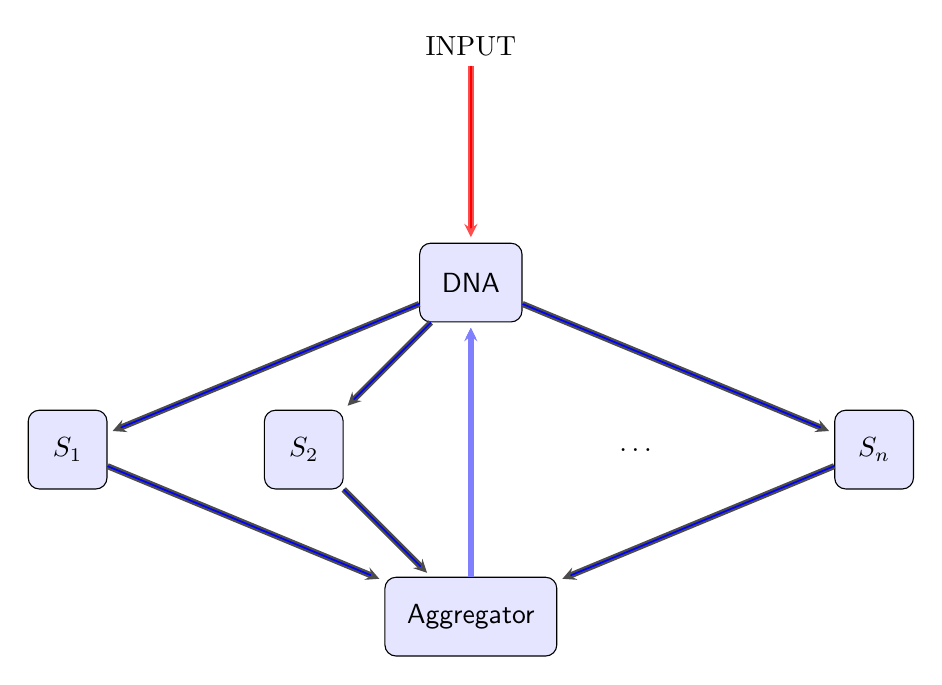
\begin{tikzpicture}[->,
    shorten >=2pt,
    >=stealth,
    node distance=3cm,
    on grid,
    state/.style={rectangle, rounded corners, draw=black, fill=blue!10, inner sep=8pt, minimum size=1cm, text centered, font=\sffamily},
    mystyle/.style={->, double=blue, thick, black!70}
    ]
    % Nodes
    \node[state] (T1) {DNA};
    \node[state] (T4) [below left=of T1] {$S_2$};
    \node[state] (T3) [left=of T4] {$S_1$};
    \node[below right=of T1] (TD) {$\dots$};
    \node[above=of T1] (TE) {INPUT};
    \node[state] (T5) [right=of TD] {$S_n$};
    \node[state] (T6) [below right=of T4] {Aggregator};
    % Edges
    \path (TE) edge [{->, double=red,  thick, red!70}] (T1);
    \path (T1) edge [mystyle] (T3);
    \path (T1) edge [mystyle] (T4);
    \path (T1) edge [mystyle] (T5);
    \path (T3) edge [mystyle] (T6);
    \path (T4) edge [mystyle] (T6);
    \path (T5) edge [mystyle] (T6);
    \path (T6) edge [{->, double=blue!50,  thin, blue!50}] (T1);
    \path (T6) edge [{->, double=blue!50,  thin, blue!50}] (T1);
    \path (T6) edge [{->, double=blue!50, thick, blue!50}] (T1);
\end{tikzpicture}
    \caption{Graph depicting the basic idea of the model.}
    \label{fig:basicmodel}
\end{figure}

The model consists of a cyclic feedback loop that can be simplified as follows. The DNA node receives a problem to solve as input and decides how many specialist nodes (referred to as stem cell nodes) and how many agents will be needed to solve that problem. Consequently, the specialist groups answer and debate within the group for an indefinite number of rounds. Once the debate rounds are over, every agent passes their answer to the aggregator node, who will be in charge of summarizing the responses from each of the $n$ stem cell nodes while still maintaining the contents. Finally, the aggregator node will pass this summary back to the DNA node, who will evaluate the responses and choose whether the final answer is satisfactory or not. If it is, then the final answer will be provided by the DNA node from the information gathered. If not, the DNA node will decide whether a rearrangement of agents or specializations is needed and have another iteration of the model until it is satisfied with the final answer. In figure \ref{fig:basicmodel}, a basic idea of the model can be observed. Each $S_i$ on the graph will be a stem cell node.

\subsection{DNA node}
The DNA node is the central and most critical component of this structure. It specifically plays two important distinctive roles:
\begin{enumerate}
    \item \textbf{Determining Specialist Groups:} When a query is received, the DNA node analyzes its complexity and requirements. Based on this analysis, it determines the optimal number of specialists needed and assigns specific roles to each. These roles are tailored to the context of the query, such as economists, politicians, or scientists, depending on the domain of the question and are freely chosen. 
    
    \item \textbf{Evaluating Specialist Outputs:} Once the specialist groups have collectively worked on the query, their results are aggregated and sent back to the DNA node. At this stage, the DNA node critically evaluates the quality of the aggregated answers and decides the next step, which, as explained previously, depends if the DNA believes if consensus has been reached and the provided answer is satisfactory (makes sense given the context and is supported by explanations).
    
\end{enumerate}
Over time, the DNA node will improve the specialization assignments based on feedback from previous interactions. By analyzing past performance and results, it can make more effective decisions about group composition, role assignment, and evaluation criteria. This self-adaptive capability ensures that the system becomes increasingly capable of addressing questions with higher precision.

\subsection{Stem Cell node}
The $n$ stem cell nodes, activated by the DNA node, play a key role in the generation of diverse and comprehensive answers to a given question. Each stem cell node operates within a designated role (e.g. economist, politician, scientist) and contributes to solving the query using specific methods and perspectives based on that particular role. The process of activating multiple stem cell nodes with different roles to answer the same question is similar to initiating weights of different distributions during deep learning. Each stem cell node approaches the question independently, making full use of its specific role to approximate the true answer from various points of view. This diversity not only can enhance the structure's ability to detect flaws by identifying significant inconsistencies between answers, but also improves comprehensiveness by integrating multiple methodologies and viewpoints into the problem-solving process. 

After generating individual responses, the specialists assigned to the same role are grouped together for a simulated discussion. Within each discussion, the specialists will review its initial answer and compare it with the responses of others for an indefinite number of rounds. Each agent then updates its response based on insights gained from others in the same stem cell node, which fosters collaborative refinement, allowing the group to collectively approximate a more accurate and robust response. 

After updating their responses, each agent makes one of two decisions:
\begin{enumerate}
    \item \textbf{Satisfactory}: If the node is confident in its updated answer, it indicates satisfaction and finalizes its response.
    \item \textbf{Dissatisfactory}: If the node finds its updated answer insufficient or considers further improvement is possible, it requests another round of discussion. In this case, the node will incorporate the refined answers of others into its own response during the next iteration.
\end{enumerate}
This iterative cycle continues until at least half of the agents in the stem cell node are satisfied.

Once the within-group discussion concludes, all the individual responses from agents in the stem cell node are aggregated into a single combined response. This aggregated answer represents a consensus or best approximation from the group and is then passed to the DNA node for evaluation.

We believe the stem cell nodes have the following advantages over single agent models:
\begin{enumerate}
    \item \textbf{Improved Accuracy}: having rounds of discussion and diverse perspectives allow errors and inconsistencies to be identified and resolved.
    \item \textbf{Dynamic Collaboration}: The mechanism of simulated discussions ensures that each agent contributes meaningfully while adapting to the contributions of others.
    \item \textbf{Scalability:} This structure can accommodate a wide range of roles, question subjects and difficulty levels, making it flexible for various types of queries.
\end{enumerate}

By building a collaborative and iterative process among specialists, stem cell nodes should ensure that the aggregated response is not only well-rounded but also robust against potential flaws or oversights. 

\subsection{Aggregator node}
The aggregator node serves as an intermediary between stem cell nodes and the DNA node, playing a crucial role in organizing and summarizing information while reducing computational overhead for the DNA node to process. The primary role of the aggregator node is to combine the responses of all specialists within a group into a single consolidated answer. This ensures that the DNA node receives a streamlined input, thereby reducing its computational burden and allowing it to focus on higher-level decision-making. The aggregator node \textbf{DOES NOT} assess the quality of individual responses or assign different weights to them. Instead, it prioritizes maintaining the originality of each contribution, which ensures that every specialist’s perspective is represented, and prevents the loss of potentially critical insights. While aiming to preserve the depth and diversity of the input, the aggregator node also considers efficiency. It combines the answers in a manner that balances the richness of the content with the need to avoid redundancy, unnecessary verbosity or repetition.


\section{Documentation on Army Hierarchy}

\subsection{Overview}

This version of the code constructs a hierarchical graph based on a custom ranking system, in this case, the U.S. Air Force rank hierarchy. Each node in the graph corresponds to a rank, represented not by its name but by a symbolic representation (e.g., stars for generals, different symbols for enlisted ranks).
The logic is similar to previous versions that used letters:

\begin{itemize}
\item     Each character in the input string (A, B, C, ..., up to V) maps to a specific rank level.
    
\item     The hierarchy is top-down, with A representing the highest rank (General of the Air Force) and subsequent letters representing progressively lower ranks.
    
\item     Sibling nodes (nodes of the same level under the same parent) are connected horizontally to show their relationship.
    
\item    The \# character breaks the sibling chain, ensuring that a node following \# will not link to its previous sibling.
\end{itemize}

\subsection{Key Concepts}

\begin{enumerate}
    \item \textbf{Hierarchy by Rank:} 
    \begin{itemize}
        \item  The code uses a predefined list of U.S. Air Force ranks.
            
        \item  Each letter (A through V) corresponds to one of the 22 ranks, from highest to lowest.
    \end{itemize}
    \item \textbf{Parent-Child Relationships:} 
    \begin{itemize}
        \item  A node representing a particular rank connects to the most recently created node of the immediately higher rank.
            
        \item  For example, if a node corresponds to 'Lieutenant General (O-9)' (C level), it connects to the most recently placed 'General (O-10)' (B level) node.
    \end{itemize}
    \item \textbf{Sibling Connections:} 
    \begin{itemize}
        \item  When multiple nodes share the same parent and appear consecutively, they link to each other as siblings.
            
        \item  This sibling link is a horizontal connection in the hierarchy, providing visual continuity and clearly grouping children of the same parent.
    \end{itemize}
    \item \textbf{Breaking Sibling Chains with \#:} 
    \begin{itemize}
        \item  The \# character acts as a reset switch for sibling connections.
            
        \item  After encountering \#, the next rank node will connect to its parent but not to its previous sibling, effectively starting a new sibling chain from that point onward.
    \end{itemize}
    \item \textbf{Symbolic Representation:} 
    \begin{itemize}
        \item  Instead of displaying the full rank names, each node is labeled with a symbolic representation.
        
        \item  For example, a 5-star rank might be shown as “$\star\star\star\star\star$”, while enlisted ranks are shown using different symbols.

        \item  This allows for a more compact and visually distinctive representation of the hierarchy.
    \end{itemize}
\end{enumerate}

\subsection{Data Structures}

\begin{itemize}
        \item  \code{rank\_symbols:} A list of symbols corresponding to each rank level. The index in this list matches the rank level derived from the character.
        \item  \code{last\_node\_of\_letter:} Maps each rank level to the last created node of that level, allowing the code to determine the correct parent node for new nodes.
        \item  \code{parent\_last\_child:} Maps a parent node to its most recently created child, enabling sibling links between consecutive children of the same parent.
    \end{itemize}


\subsection{Key Concepts}

\begin{enumerate}
    \item \textbf{Input String Parsing:} 
    \begin{itemize}
        \item  The input string is examined character by character.
        \item Letters (A to V) are converted to a rank level index and thus to a rank symbol.
        \item Nodes are created and linked to their parents (if not top-level).
        \item Sibling links are created between consecutive siblings unless a \# break occurs.
    \end{itemize}
    \item \textbf{\# Reset Mechanism:} 
    \begin{itemize}
        \item  On encountering \#, sibling linking information is cleared.
        \item The subsequent node after \# connects only to its parent, not its previous sibling.
        \item After placing that node, sibling linking resumes normally for subsequent nodes.
    \end{itemize}
    \item \textbf{Graph Rendering:} 
    \begin{itemize}
        \item  The code uses \code{pygraphviz} for hierarchical layout (top-to-bottom) and \code{matplotlib} for visualization.
        \item Each node displays a rank symbol.
        \item Edges are drawn without arrowheads, focusing on hierarchy and sibling structure rather than direction.
    \end{itemize}
    \item \textbf{Checking Order with \code{check\_string\_allowed}:} 
    \begin{itemize}
        \item  Before building the graph, you can run \code{check\_string\_allowed(input\_string)} to ensure the string introduces ranks in proper alphabetical order of first appearance.
        \item Once all letters are introduced in the correct order, they can reappear in any sequence.
    \end{itemize}
\end{enumerate}

\subsection{Example With Visualizations}
\begin{itemize}
        \item  Consider an input "ABBCABB":
        \begin{itemize}
            \item[--] A might represent the top rank (General of the Air Force).
            \item[--] B corresponds to the next rank (General, O-10).
            \item[--] Additional Bs connect under A and link to each other as siblings.
            \item[--] Later, encountering C would connect to the last B.
            \item[--] Another A introduces a new top-level node, and subsequent Bs under that A form another sibling chain.
        \end{itemize}
        \item Adding a \# (e.g., "AB\#B") breaks the sibling chain, so the second B after \# does not form a sibling link with the previous B.
\end{itemize}

\begin{figure}
    \centering
    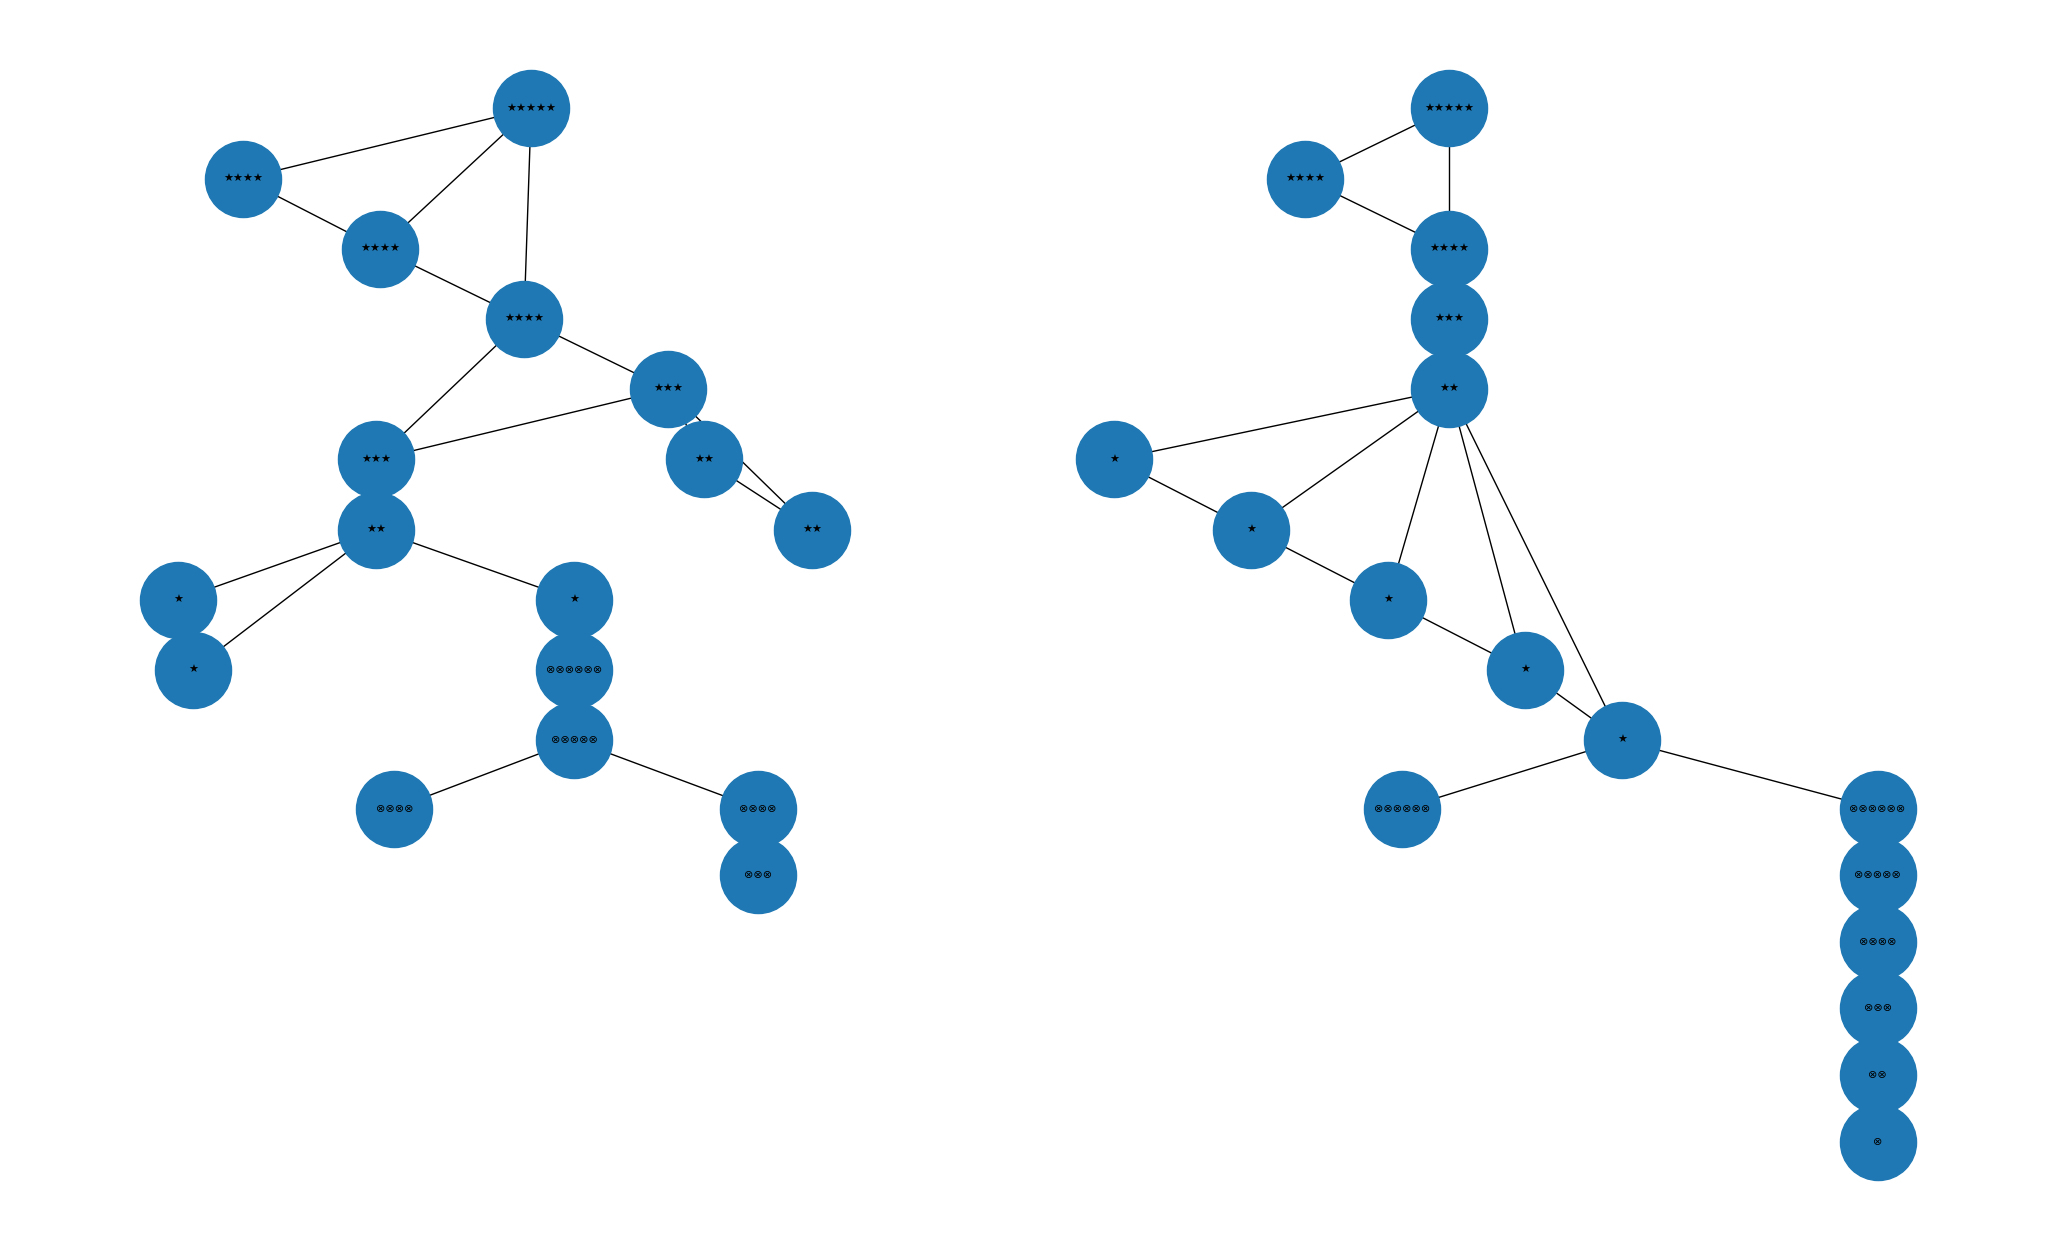
\includegraphics[scale=.3]{report1/img/documentation/test_structure_output.png}
    \caption{Example of the structure for input "ABBBCDDCDEE\#EFGH\#HIABBCDEEEEEF\#FGH\#I\#J\#K"}
    \label{fig:teststructureoutput}
\end{figure}

\begin{figure}
    \centering
    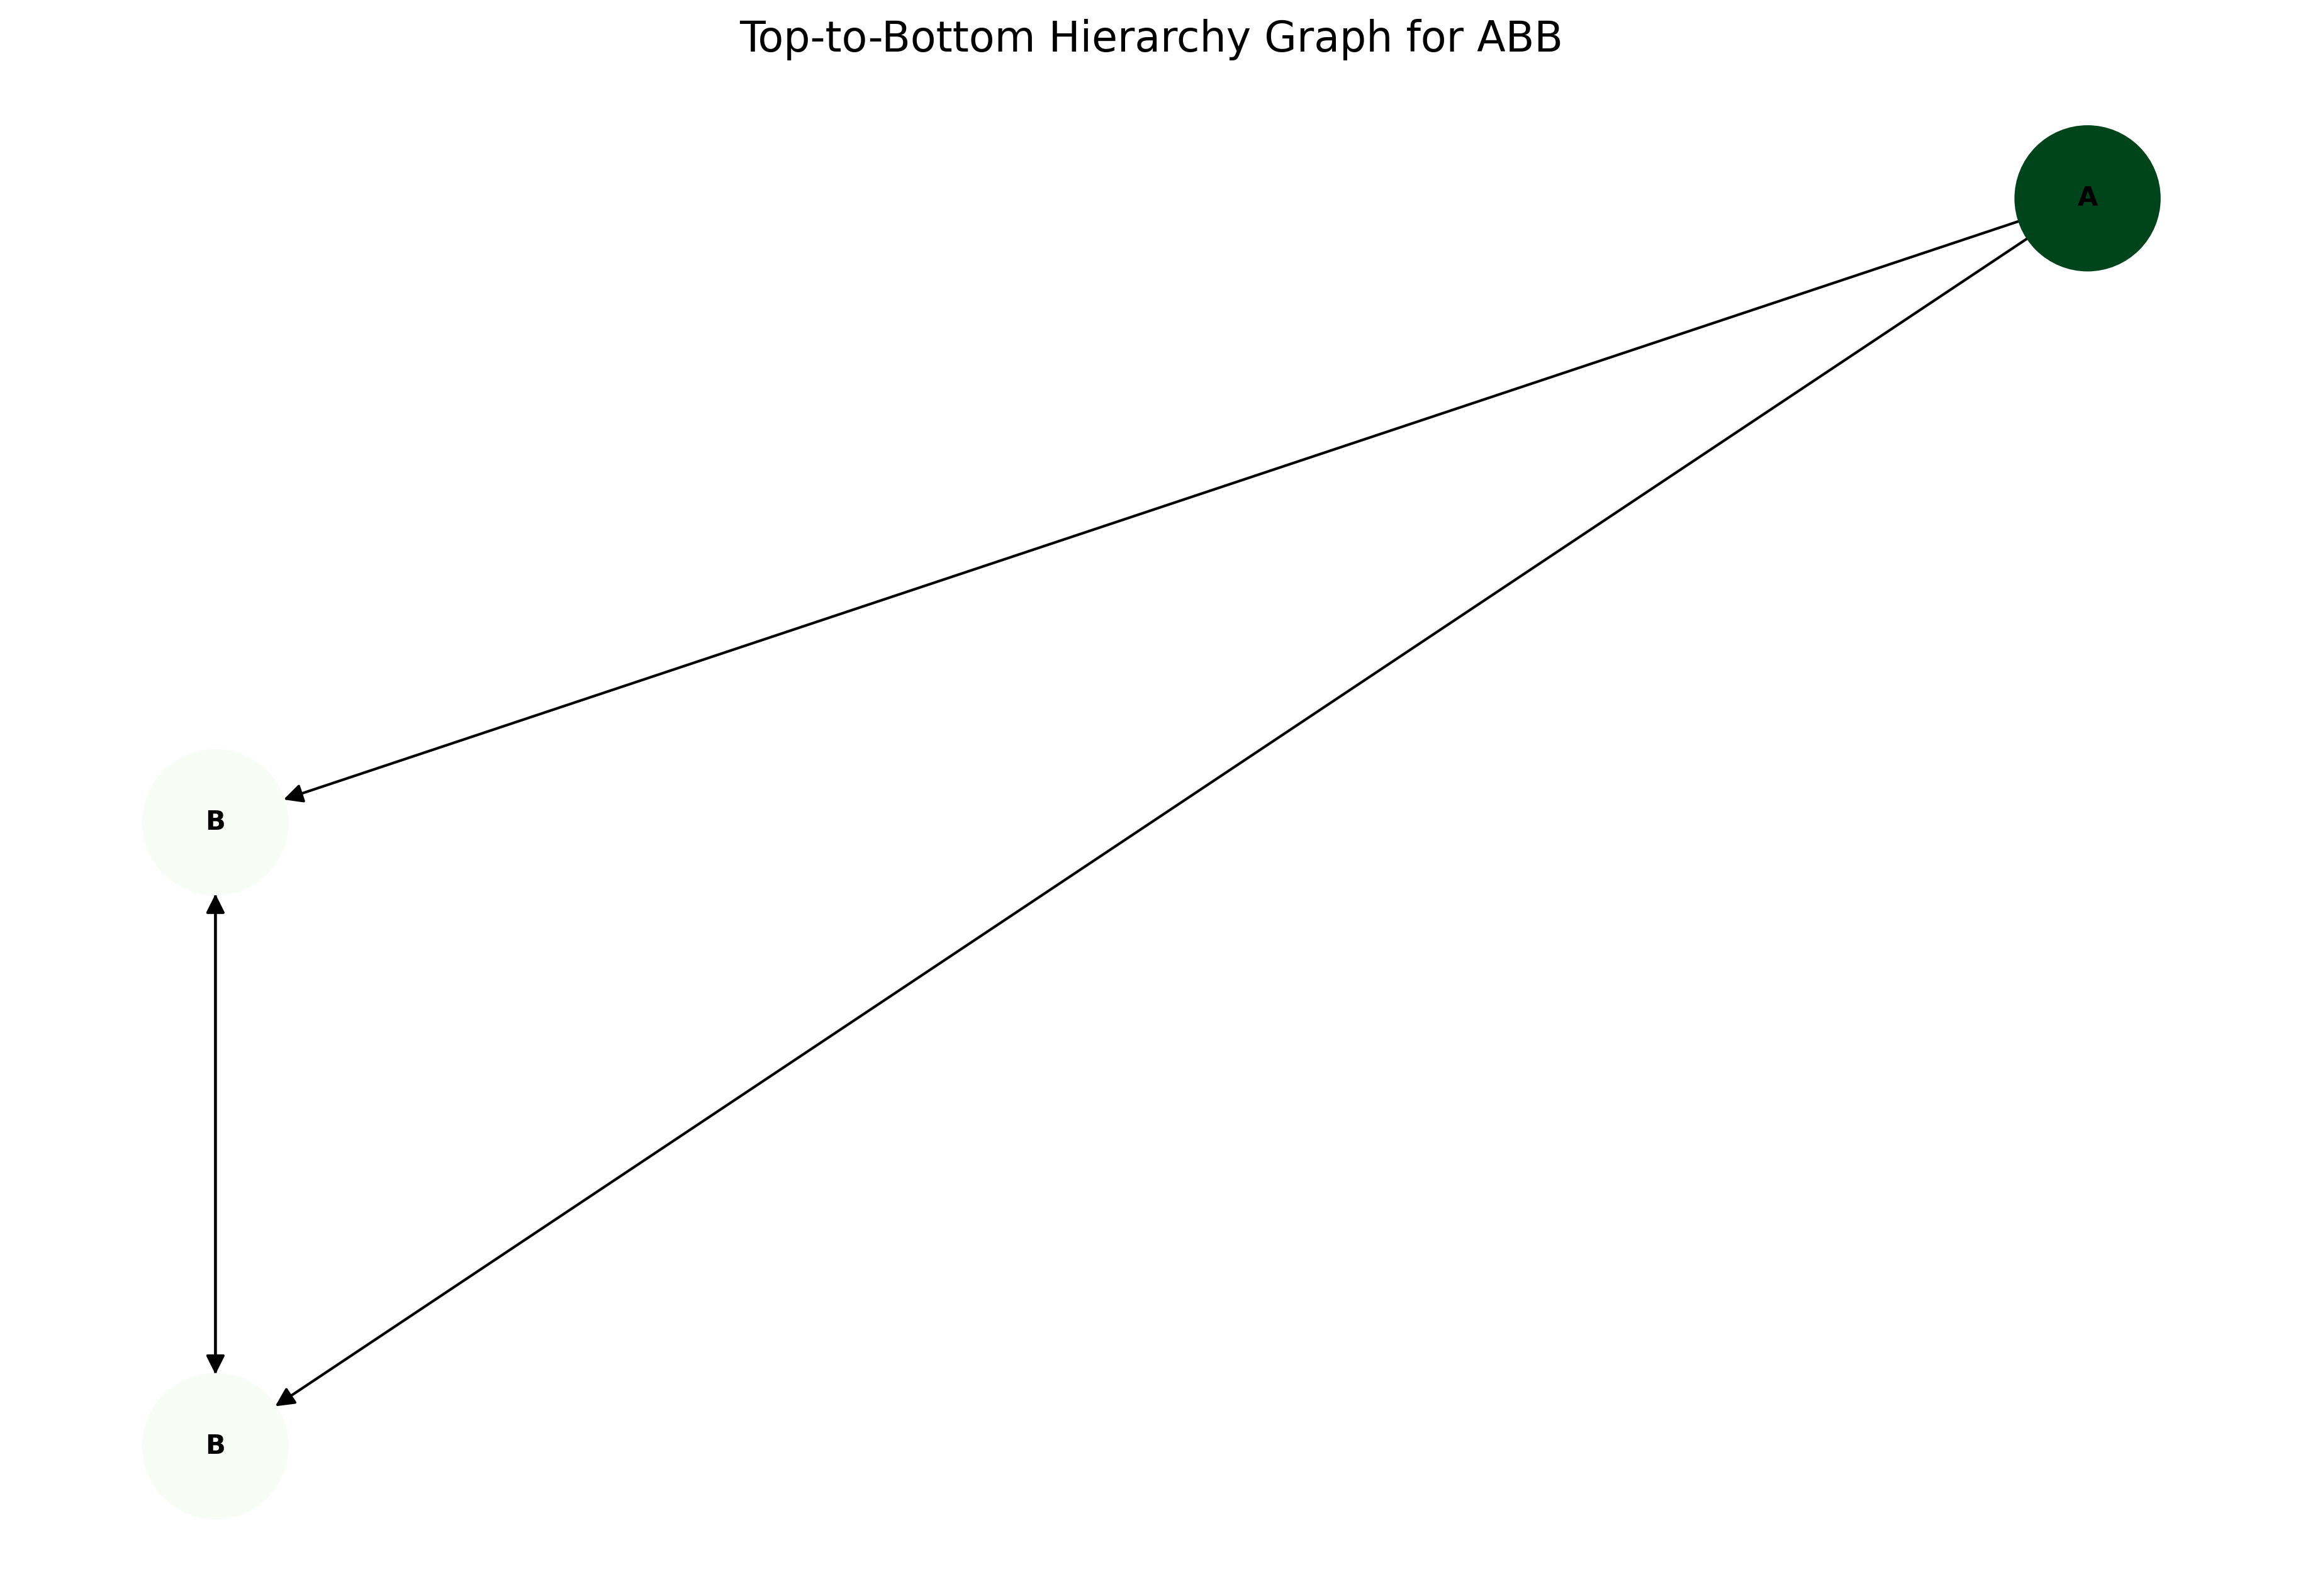
\includegraphics[scale=.5]{report1/img/documentation/ABB.png}
    \caption{Example of the structure for input "AB\#B"}
    \label{fig:abb}
\end{figure}
\pagebreak 

\section{Conclusion}
\label{sec:conclusion}

This study demonstrates that incorporating a hierarchical communication topologies into a multi-agent debate system enhances accuracy compared to zero-shot reasoning. Furthermore, our analysis suggests that redundancy in communication may strengthen the system’s self-correcting ability, leading to more reliable outcomes.

\newpage

% sections
% \nocite{*}
\bibliographystyle{unsrt}
\bibliography{bib/main.bib}

\end{document}
